\def\partcell{
--++(1,0)--++(0,1)--++(-1,0)--cycle ++(0.5,-1.1) node[anchor=south]
}

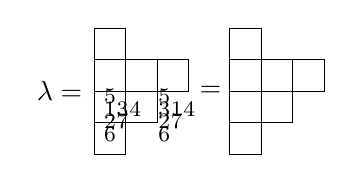
\begin{tikzpicture}[scale=0.4]
  \draw (-1.1,0) node {$\lambda=$};
  \foreach \x/\b in {0/1,1/3,2/4} \draw (\x,0) \partcell {\footnotesize\b};
  \foreach \x/\b in {0/2,1/7} \draw (\x,-1) \partcell {\footnotesize\b};
  \foreach \x/\b in {0/6} \draw (\x,-2) \partcell {\footnotesize\b};
  \foreach \x/\b in {0/5} \draw (\x,1) \partcell {\footnotesize\b};
  \draw (3.7,0) node {$=$};
  \foreach \x/\b in {0/3,1/1,2/4} \draw ++(4.3,0) ++(\x,0) \partcell {\footnotesize\b};
  \foreach \x/\b in {0/2,1/7} \draw ++(4.3,0) ++(\x,-1) \partcell {\footnotesize\b};
  \foreach \x/\b in {0/6} \draw ++(4.3,0) ++(\x,-2) \partcell {\footnotesize\b};
  \foreach \x/\b in {0/5} \draw ++(4.3,0) ++(\x,1) \partcell {\footnotesize\b};
\end{tikzpicture}
